\documentclass[tikz,border=10pt]{standalone}
\usepackage{tikz}
\usepackage{mathptmx}

\begin{document}
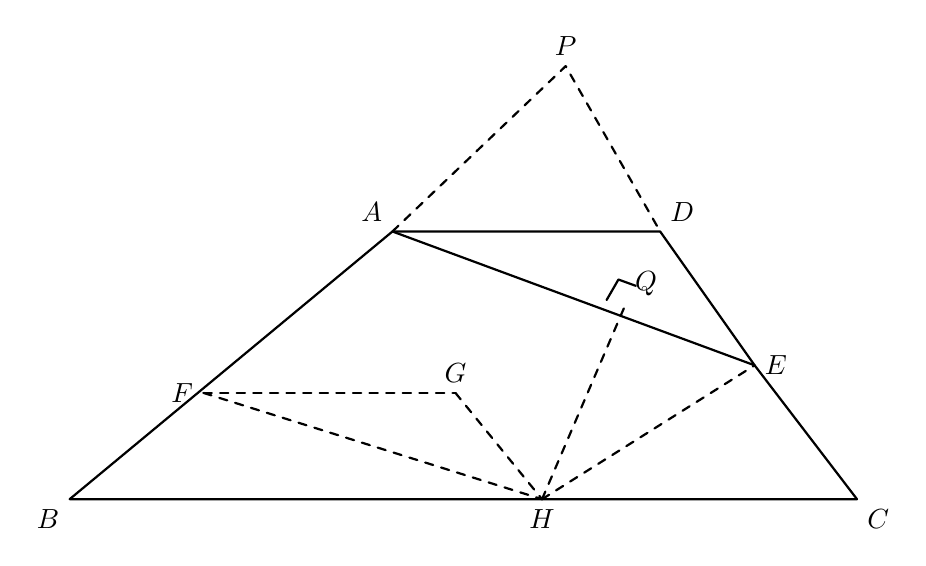
\begin{tikzpicture}[line cap=round,line join=round,thick]

% Coordinates
\coordinate (B) at (0,0);
\coordinate (C) at (10,0);
\coordinate (A) at (4.1,3.4);
\coordinate (D) at (7.5,3.4);
\coordinate (E) at (8.7,1.7);
\coordinate (P) at (6.3,5.5);
\coordinate (F) at (1.7,1.35);
\coordinate (G) at (4.9,1.35);
\coordinate (H) at (6.0,0.0);
\coordinate (Q) at (7.05,2.45);

% Solid outer figure
\draw (B) -- (A) -- (D) -- (E) -- (C) -- (B);

% Solid interior segment
\draw (A) -- (E);

% Dashed top triangle extensions
\draw[dashed] (A) -- (P) -- (D);

% Dashed interior segments
\draw[dashed] (F) -- (G);
\draw[dashed] (F) -- (H);
\draw[dashed] (G) -- (H);
\draw[dashed] (H) -- (E);
\draw[dashed] (H) -- (Q);

% Right-angle mark at Q between AE and HQ
\coordinate (Qx) at (6.82,2.53);
\coordinate (Qy) at (6.97,2.79);
\coordinate (Qr) at (7.19,2.71);
\draw (Qx) -- (Qy) -- (Qr);

% Labels
\node[below left] at (B) {$B$};
\node[below right] at (C) {$C$};
\node[above left] at (A) {$A$};
\node[above right] at (D) {$D$};
\node[right] at (E) {$E$};
\node[above] at (P) {$P$};
\node[left] at (F) {$F$};
\node[above] at (G) {$G$};
\node[below] at (H) {$H$};
\node[above right] at (Q) {$Q$};

\end{tikzpicture}
\end{document}
